% FleetMem paper draft — Overleaf-ready.
% Compile: pdfLaTeX (or XeLaTeX). Class: acmart (available on Overleaf).
\documentclass[sigconf,anonymous]{acmart}

\usepackage{booktabs}
\usepackage{graphicx}
\usepackage{multirow}
\usepackage{xspace}

\settopmatter{printacmref=false}
\setcopyright{none}
\renewcommand\footnotetextcopyrightpermission[1]{}
\pagestyle{plain}

\newcommand{\sys}{FleetMem\xspace}
\newcommand{\smb}{SMB\xspace}

\title{FleetMem: Budget-Constrained Semantic Memory for Always-On Video Fleets}

\begin{document}

\begin{abstract}
Always-on camera fleets need persistent, queryable memory of what happened, but existing approaches force a choice between two unbudgeted extremes: retaining model-internal key--value state, which is opaque, per-stream, and grows at gigabytes per stream-hour, or building semantic indexes with unconditional time-driven writes whose compute cost is never reported. Neither paradigm treats memory as a resource with a budget. We present \sys, a serving system that maintains a queryable semantic memory over many live camera streams under explicit GPU and storage budgets. \sys contributes four budgeted policies: event-driven memory writes gated by a cheap tier-1 signal; coverage-aware eviction with tombstones that convert deletion into compression; a fleet admission controller that sheds low-salience writes under overload; and a calibrated query path that can abstain. We also contribute SMB, a 300-query surveillance memory benchmark with ground-truth evidence spans over UCF-Crime, XD-Violence, and ShanghaiTech. On 4$\times$V100 hardware, \sys answers existence queries at 0.95 accuracy with a write cost of 244 GPU-s per stream-hour and 1.13\,MB per stream-day --- beating every baseline on every accuracy metric while using $\sim$2$\times 10^4\times$ less storage than even aggressively compressed KV-cache retention (MuKV at 3/4 removal) and $\sim$5$\times$ less write compute than time-driven captioning. Under fleet overload, admission control preserves timely memory for high-salience events at 10--20$\times$ the rate of fair queueing. All measurements are reproducible; every run is pinned by configuration, environment, and code state.
\end{abstract}

\maketitle

\section{Introduction}
\label{sec:intro}

Camera fleets are among the largest producers of continuous data in the world, and the questions their operators ask are simple to state: \emph{``Did anyone enter the loading dock after 22:00?''}, \emph{``When did the fight start?''}, \emph{``Show me all robberies this week.''} Answering such questions requires a system that watches many always-on streams and maintains a \emph{persistent, queryable memory} of what happened. The recent wave of video-capable language models~\cite{qwen25vl,internvl,llavaov} makes the semantics attainable; what does not yet exist is the \emph{system} that makes them affordable at fleet scale.

We audited the two existing paradigms for memory over video (Section~\ref{sec:gap}) and found that both are defined by the absence of budgets:

\paragraph{KV-state memory.} Streaming video-LLM systems retain key--value cache tensors per stream~\cite{rekv,livevlm,streammem,streamingvlm}. Full-fidelity retention costs 18.8\,GB per stream-hour at 7B quality~\cite{rekv} --- a 100-camera fleet would need $\sim$45\,TB/day --- and ReKV itself calls this growth ``unsustainable'' for surveillance. Compressed variants~\cite{livevlm,streammem} cap a per-stream token budget as an accuracy hyperparameter, but the memory remains opaque (not queryable across streams), model-bound, and evaluated only on single streams of minutes to an hour.

\paragraph{Semantic memory.} A parallel line builds textual/graph memory: Avas captions \emph{every 3-second chunk} unconditionally~\cite{avas}, VideoRAG every 30-second clip~\cite{videoraghkuds}, WorldMM at fixed intervals while retaining every sampled frame~\cite{worldmm}, and the VideoDB report prices a VLM call every 5 seconds per stream~\cite{videodb}. None reports bytes per stream-hour, GPU-seconds per camera-hour, or any accuracy-vs-cost operating curve; the VideoDB report explicitly defers cost measurement to future work. And none evaluates more than one stream: Avas's own throughput numbers show a single stream nearly saturating one RTX\,3090.

Meanwhile, a measurement fact about the workload goes unexploited: surveillance is \emph{mostly uneventful}. In UCF-Crime only 7.8\% of clips are anomalous~\cite{ucfcrime}, and our measurements (Appendix~\ref{app:e0}) show temporal redundancy concentrates within one minute. Time-driven writes therefore spend the dominant cost narrating static footage.

This paper presents \sys, a serving system that treats semantic memory as a \emph{budgeted resource}. Given $N$ camera streams, one GPU server, and explicit GPU/storage budgets, \sys maintains a tiered memory (metadata, narrated event records, embeddings, raw-footage pointers) and answers natural-language queries with evidence, bounded latency, and measured cost. Its four policies are each backed by a measurement that prior work does not report:

\begin{itemize}
\item \textbf{Event-driven writes} (what deserves memory at all): a cheap tier-1 salience signal gates expensive VLM narration, cutting write compute $\sim$3$\times$ vs.\ time-driven captioning at equal event recall (Section~\ref{sec:exp-write}).
\item \textbf{Coverage-aware eviction with tombstones} (what survives): eviction becomes compression --- evicted events leave compact stubs that preserve aggregate answerability at $\sim$2\% storage (Section~\ref{sec:exp-eviction}).
\item \textbf{Fleet admission control} (whose writes happen under overload): ordering alone provably does nothing under saturation --- priority queueing is statistically indistinguishable from FCFS in our measurements --- while shedding low-salience writes holds the freshness SLO for high-salience events at 10--20$\times$ the rate of fair queueing (Section~\ref{sec:exp-fleet}).
\item \textbf{Calibrated query path with abstention} (when to answer): retrieval over the memory, optional asymmetric verification against raw footage, and an explicit not-answerable outcome (Section~\ref{sec:design-query}).
\end{itemize}

We evaluate \sys on 4$\times$Tesla V100 hardware against runnable baselines --- ReKV~\cite{rekv}, LiveVLM-lineage compression~\cite{livevlm,mukv}, time-driven captioning (an Avas-style policy)~\cite{avas}, TASTI-style appearance indexes~\cite{tasti}, and direct VLM reading --- on \smb, our new 300-query surveillance memory benchmark built from UCF-Crime, XD-Violence, and ShanghaiTech~\cite{ucfcrime,xdviolence,shanghaitech} with ground-truth evidence spans and a QC-checked answer key. \sys leads every accuracy metric among memory systems at $\approx$0 GPU-s per query, with 1.13\,MB/stream-day storage versus $\sim$103\,GB/stream-day for full-fidelity KV retention at 0.5B scale and $\sim$24\,GB/stream-day even at MuKV's aggressive 3/4-removal setting~\cite{mukv,rekv}.

\paragraph{Contributions.}
\begin{enumerate}
\item \textbf{\sys}, the first video memory system with explicit GPU/storage budgets, budgeted event-driven writes, eviction-with-tombstones, fleet admission control, and abstaining queries (Sections~\ref{sec:design}).
\item \textbf{\smb}, the first query/memory benchmark over always-on surveillance video, with five query types, ground-truth evidence, and an independent QC pass (Section~\ref{sec:exp-smb}).
\item \textbf{A cost-accounting methodology} (GPU-s/camera-hour, MB/stream-day, accuracy-vs-cost frontiers) applied uniformly to all systems, including baselines (Sections~\ref{sec:exp-setup}--\ref{sec:exp-baselines}).
\item \textbf{Measured negative results with design consequences}: appearance embeddings fail as event memory in-system (Section~\ref{sec:exp-tasti}); priority ordering without admission control is useless under saturation (Section~\ref{sec:exp-fleet}); VLMs are near-useless as online anomaly \emph{scorers} but effective as gated \emph{narrators} (Appendix~\ref{app:e0}).
\end{enumerate}

\section{Related Theory}
\label{sec:related}

\sys sits at the intersection of four research lines. For each, we summarize the theory and --- critically for a systems paper --- what each line measures and what it does not.

\subsection{Video analytics systems (the cost-aware lineage)}
\label{sec:related-vas}

The classical lineage optimizes declarative queries over video with cheap-model cascades and indexes. NoScope cascades frame-difference detectors and per-stream proxy CNNs before an expensive target model~\cite{noscope}; Focus builds a coarse ingest-time index and spends the expensive model only on promising index clusters at query time~\cite{focus}; BlazeIt accelerates aggregation and limit queries via control-flow sampling~\cite{blazeit}; TASTI builds a task-agnostic \emph{semantic index} --- embedding buckets whose cluster representatives stand in for full inference~\cite{tasti}; SUPG adds proxy scores with statistical guarantees~\cite{supg}. Resource allocation across streams appears in VideoStorm (quality/resource knob profiles over thousands of streams)~\cite{videostorm}, Chameleon (periodic re-profiling exploiting temporal and cross-camera correlation)~\cite{chameleon}, and VideoEdge (hierarchical cluster placement for camera fleets)~\cite{videoedge}. MIRIS integrates query processing into object tracking~\cite{miris}; Panorama supports unbounded-vocabulary queries over video~\cite{panorama}; VStore manages fidelity tiers of the stored video itself~\cite{vstore}.

This lineage established cost-aware query processing, and we adopt its evaluation discipline (accuracy at a cost target). But it predates open-vocabulary semantics: its queries are fixed-schema (object classes, tracks, counts), its indexes are appearance embeddings, and none of it persists a \emph{memory} that natural-language queries can address. Our TASTI-lite baseline (Section~\ref{sec:exp-tasti}) instantiates this lineage's strongest idea --- the embedding index --- against our text-and-tag memory, and loses on event semantics, consistent with the appearance-signature failure we measured previously (Appendix~\ref{app:e0}).

\subsection{Streaming video LLMs and KV-state memory}
\label{sec:related-kv}

A second line adapts video-LLMs to online streams. VideoLLM-online introduced streaming dialogue training for continuous video~\cite{videollmonline}; Flash-VStream added a memory-based streaming architecture and the RVS benchmarks~\cite{flashvstream}; Dispider disentangles perception, decision, and reaction timing~\cite{dispider}; StreamingVLM sustains infinite commentary with a fixed KV window (512 text tokens + 16\,s of vision) and recency eviction~\cite{streamingvlm}. The KV-retrieval/compression sub-line manages the cache explicitly: ReKV offloads full-fidelity per-frame KV to RAM/disk and retrieves top-$r$ frames per query~\cite{rekv}; LiveVLM compresses online via vision-sink bucketing and retrieves position-agnostic KV pages~\cite{livevlm}; StreamMem prunes to a query-agnostic saliency budget~\cite{streammem}; MuKV compresses at multiple temporal granularities~\cite{mukv}; WeaveTime retrieves past KV via uncertainty triggers~\cite{weavetime}; V-Rex accelerates streaming KV retrieval in hardware~\cite{vrex}. Venus separates memory across an edge--cloud split~\cite{venus}; on the serving side, PagedAttention/vLLM established paged KV management for LLM inference generally~\cite{vllm}, and Stream2LLM addresses scheduling of streaming LLM workloads~\cite{stream2llm}; CodecSight exploits codec signals to cut streaming VLM inference~\cite{codecsight}.

Two properties of this line matter for us. First, its memory is \emph{model-internal state}: not queryable across streams, not portable, and --- at 18.8\,GB/stream-hour for full fidelity at 7B scale~\cite{rekv} --- economically unbounded; ReKV's own appendix names surveillance-scale growth ``unsustainable.'' Second, its evaluation is single-stream and budget-free: token caps are accuracy hyperparameters, and no work in this line reports cost per stream-hour, a fleet model, or an accuracy-vs-cost frontier. We reuse this line as per-stream \emph{components} and as baselines (Sections~\ref{sec:exp-baselines}, \ref{sec:exp-generality}), and our design leaves a slot for an optional KV tier for fine-grained detail (Section~\ref{sec:discussion}).

\subsection{Semantic memory and retrieval over video}
\label{sec:related-semantic}

A third line builds queryable semantic artifacts. VideoRAG constructs a knowledge graph plus text and per-clip visual embeddings over a video corpus, with every 30-s clip captioned and every video transcribed~\cite{videoraghkuds}; an independent NeurIPS variant augments retrieval with OCR/ASR/detection side channels~\cite{videoragneurips}. WorldMM maintains episodic, semantic, and visual memories at four temporal scales, including retaining every sampled frame, driven by frontier API models~\cite{worldmm}. Avas builds an event knowledge graph over continuous streams with agentic tree-search querying~\cite{avas}. The VideoDB report articulates persistent visual memory as layered, analyzer-defined indexes with live streams as first-class sources~\cite{videodb}. LazyVLM decomposes multi-frame queries neuro-symbolically~\cite{lazyvlm}; D\'ej\`a Vu reuses ViT embeddings across temporally redundant frames at query time~\cite{dejavu}; Zelda performs VLM top-$k$ video queries~\cite{zelda}; Lava revisits the classic cascade lineage with language-driven traffic analytics~\cite{lava}; agentic-memory variants (M3-Agent, StreamMeCo, MAGIC-Video) compress long-term agent memory for streaming video~\cite{m3agent,streammeco,magicvideo}.

Every one of these systems writes memory \emph{time-driven and unconditionally}, grows it \emph{unboundedly}, and evaluates \emph{accuracy-only} on a single stream or offline corpus. Avas's throughput (2.5\,FPS indexing vs.\ 2\,FPS input on one RTX\,3090) implies one stream nearly saturates one GPU; VideoDB defers cost measurement explicitly. To our knowledge no published system budgets memory writes, evicts under a storage budget, schedules writes across a fleet, or reports an accuracy-vs-cost frontier. Section~\ref{sec:gap} tabulates this.

\subsection{Video anomaly detection}
\label{sec:related-vad}

Weakly-supervised VAD provides our tier-1 signal and evaluation substrates. UCF-Crime introduced the 13-category surveillance benchmark with 7.8\% anomalous clips~\cite{ucfcrime}; ShanghaiTech offers a 12--13-camera campus setting~\cite{shanghaitech}; XD-Violence adds audio-visual violence detection with 145{,}612 test clips~\cite{xdviolence}. VadCLIP adapts CLIP to weakly-supervised VAD~\cite{vadclip}; cascade designs gate an expensive VLM stage per stream (MemoVAD~\cite{memovad}); Holmes-VAU and VERA bring VLM-based anomaly understanding~\cite{holmesvau,vera}; UCVL benchmarks MLLMs on crime-surveillance tasks~\cite{ucvl}. Our prior measurement study (Appendix~\ref{app:e0}) showed VLM escalation adds $\Delta$AUC\,$\approx 0$ over a strong tier-1 scorer --- which is why, in \sys, the VLM \emph{narrates} gated events rather than \emph{scoring} them, and why category labels come from tier-1 while narrations carry description.

\subsection{Benchmarks for streaming video understanding}
\label{sec:related-bench}

OVO-Bench and its successor OVO-S-Bench evaluate real-time and backward-looking streaming QA on egocentric and web video~\cite{ovobench,ovosbench}; StreamingBench covers 900 videos with 4.5K QA pairs~\cite{streamingbench}; Video-MME, LVBench, MLVU, and LongVideoBench cover offline long-video QA~\cite{videomme,lvbench,mlvu,longvideobench}. None targets always-on \emph{surveillance} streams (no audio, sparse events, multi-camera topology), none carries ground-truth evidence spans suited to memory evaluation, and none is cost-instrumented. This gap motivates \smb (Section~\ref{sec:exp-smb}).

\section{Gap Analysis and Problem Formulation}
\label{sec:gap}

\subsection{The gap, stated precisely}
\label{sec:gap-matrix}

We read the eight closest systems in full and tabulated what each stores, when it writes, whether it budgets or evicts, whether it models multiple streams, and whether it accounts cost (details in Appendix~\ref{app:profiles}). Table~\ref{tab:gap} is the result. Four verifiable absences define the open problem:

\begin{enumerate}
\item \textbf{No budget abstraction.} No system takes a GPU, storage, or dollar budget as input and reports accuracy as a function of it. KV-line token caps~\cite{livevlm,streammem,streamingvlm} are per-stream accuracy hyperparameters, not system budgets; the semantic line~\cite{avas,videoraghkuds,worldmm,videodb} reports no cost model at all.
\item \textbf{Every write is time-driven.} Every frame (ReKV, 0.5\,FPS), every 3\,s (Avas), every 5\,s (VideoDB), every 30\,s (VideoRAG) is processed identically regardless of content. In a regime where 7.8\% of clips are anomalous and 94.4\% of temporal redundancy is sub-minute (Appendix~\ref{app:e0}), unconditional writes spend the dominant cost on static footage.
\item \textbf{No fleet model.} Zero multi-stream evaluation, zero contention, zero write scheduling. The two available data points are stark: full-fidelity KV retention implies $\sim$45\,TB/day for a 100-camera fleet~\cite{rekv}, and one Avas-style indexer nearly saturates one consumer GPU on one stream~\cite{avas}.
\item \textbf{No cost accounting.} Nobody reports GPU-seconds per camera-hour, bytes per stream-day, or accuracy-vs-cost curves. The field's metrics (accuracy, win-rate) are cost-blind.
\end{enumerate}

\begin{table}[t]
\centering
\caption{Gap matrix: capabilities of the eight closest systems, verified against their papers (Appendix~\ref{app:profiles}). ``KV'' = model-internal KV tensors only. $\dagger$: per-stream token cap as hyperparameter, not a system budget.}
\label{tab:gap}
\small
\begin{tabular}{@{}lcccccc@{}}
\toprule
System & Budgeted writes & Event-driven & Eviction & Fleet & Cost accounting & Queryable memory \\
\midrule
ReKV~\cite{rekv} & \texttimes & \texttimes & \texttimes & \texttimes & partial (GB/h) & KV only \\
LiveVLM~\cite{livevlm} & $\dagger$ & \texttimes & KV pruning & \texttimes & ratios only & KV only \\
StreamMem~\cite{streammem} & $\dagger$ & \texttimes & KV pruning & \texttimes & \texttimes & KV only \\
StreamingVLM~\cite{streamingvlm} & window & \texttimes & recency & \texttimes & \texttimes & \texttimes \\
Avas~\cite{avas} & \texttimes & \texttimes & \texttimes & \texttimes & spot numbers & graph+text \\
VideoRAG~\cite{videoraghkuds} & \texttimes & \texttimes & \texttimes & \texttimes & \texttimes & graph+emb. \\
WorldMM~\cite{worldmm} & \texttimes & \texttimes & \texttimes & \texttimes & \texttimes & KG+frames \\
VideoDB~\cite{videodb} & \texttimes & \texttimes & \texttimes & \texttimes & \texttimes & artifacts \\
\midrule
\sys (ours) & \checkmark & \checkmark & \checkmark & \checkmark & \checkmark & tiered \\
\bottomrule
\end{tabular}
\end{table}

\subsection{Problem formulation}
\label{sec:formulation}

\textbf{Setting.} $N$ always-on camera streams $s_1,\dots,s_N$ share one GPU server with per-tier compute capacities and a storage allowance. A stream is an unbounded sequence of chunks; a small subset of chunks belong to \emph{events} worth remembering. Queries $q$ arrive over the fleet's lifetime; each asks about the past (retrospective) or the live edge (any-time), scoped to a video, the corpus, or the fleet.

\textbf{Budgets.} The system receives: (i) a \emph{write budget} $B_W$ in GPU-s per stream-hour (how much compute memory-writing may consume, fleet-wide); (ii) a \emph{storage budget} $B_S$ in bytes per stream-day (how much memory may persist); (iii) a \emph{query budget} $B_Q$ in GPU-s per query (verification effort allowed at answer time).

\textbf{Memory.} A memory $\mathcal{M}$ is a set of records $r = (\text{stream}, \text{span}, \text{salience}, \text{tag}, \text{narration}, \text{embedding}, \text{tombstone?})$ written by the write path, evicted under $B_S$ by the eviction policy, and read by the query path.

\textbf{Objective.} Maximize query accuracy under budgets, with a freshness constraint:
\begin{equation}
\max_{\text{policies}} \; \mathrm{Acc}(\mathcal{M}, \mathcal{Q}) \quad \text{s.t.} \quad \mathrm{GPU\text{-}s/stream\text{-}h} \le B_W,\;\; \mathrm{bytes/stream\text{-}day} \le B_S,\;\; \mathrm{GPU\text{-}s/query} \le B_Q,
\end{equation}
and, for always-on operation, \emph{memory freshness} --- the virtual time from event occurrence to its record being written --- must satisfy an SLO (we use 60\,s) even under bursty load.

\textbf{Query types and metrics} (instantiated by \smb, Section~\ref{sec:exp-smb}): \emph{existence} (accuracy), \emph{negation} (false-alarm rate; the system must not hallucinate absent events), \emph{temporal localization} (tIoU against ground-truth spans), \emph{retrieval} (Recall@$k$ / average precision over a relevant set), \emph{cross-camera} (set/count accuracy over cameras). All are reported \emph{against cost}, never alone.

\textbf{Why prior formulations do not apply.} Single-stream KV systems optimize per-stream accuracy under a VRAM cap; semantic-memory systems optimize corpus QA accuracy; classic video analytics optimizes fixed-schema query latency. None can express ``$N$ streams, $B_W$ GPU-s/h, $B_S$ bytes/day, maximize event-recall-weighted query accuracy with 60\,s freshness,'' which is the operator's actual problem.

\section{System Design}
\label{sec:design}

\begin{figure*}[t]
\centering
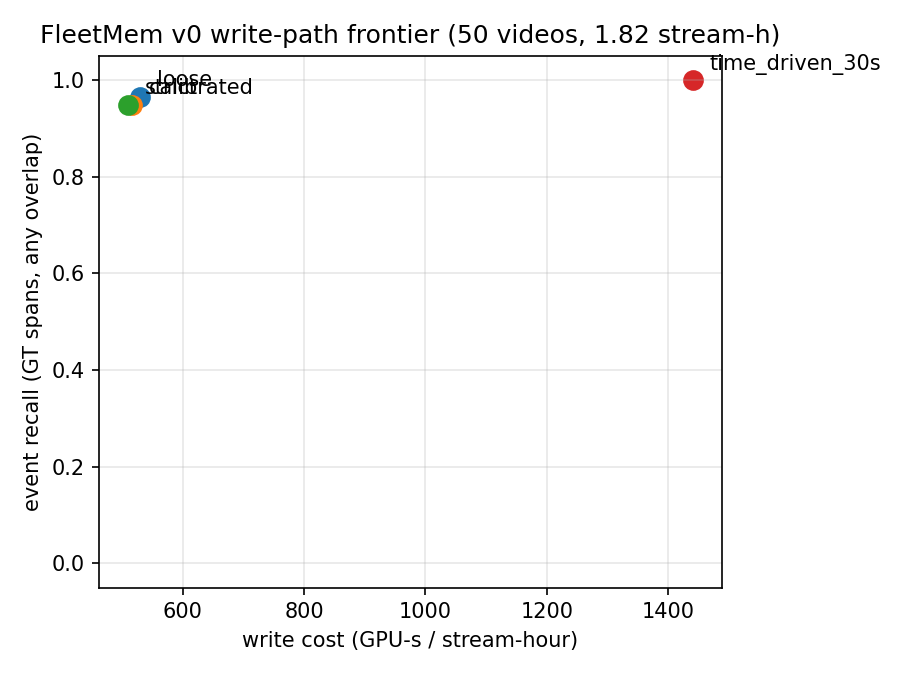
\includegraphics[width=0.9\textwidth]{figures/write_frontier.png}
\caption{Event-recall vs.\ write cost and storage on a 50-video stratified subset (59 ground-truth events). Event-driven gates reach recall 0.949--0.966 at 509--530 GPU-s/stream-hour (stride-1 tier-1 charge; stride 4 subtracts 264 GPU-s/stream-hour, Section~\ref{sec:exp-write}) and $\sim$1.2\,MB/stream-day; time-driven 30-s captioning (the Avas-style policy) reaches 1.000 at 1{,}442 GPU-s/stream-hour and 7.7\,MB/stream-day. Gate separation is small because tier-1 scores are bimodal on this subset (Section~\ref{sec:exp-write}).}
\label{fig:write-frontier}
\end{figure*}

\sys comprises a per-stream \emph{write ladder}, a \emph{tiered memory}, a \emph{fleet arbiter}, and a \emph{query path} (Figure~\ref{fig:write-frontier} previews the write economics). Every design choice below is justified by a measurement; cross-references point to the evidence.

\subsection{The write ladder: event-driven memory writes}
\label{sec:design-write}

Each stream is processed by a three-tier ladder; each tier gates the next, so expensive computation runs only where cheaper computation says it matters.

\paragraph{Tier 0: decode.} Frames are decoded on CPU (measured: 25{,}482 frames/s across 16 cores; 0.6\% of the GPU budget; Appendix~\ref{app:e0}). Decode is never the bottleneck at our scale and is excluded from GPU accounting.

\paragraph{Tier 1: salience.} A weakly-supervised anomaly scorer (VadCLIP~\cite{vadclip}, reproduced to within 0.0001 of its published AUC in our prior study) produces a per-clip score stream. Two measurements justify using it as a gate: tier-1 is 4--8$\times$ oversampled for detection (stride 4 costs $-$0.0014 AUC at 4$\times$ less compute), and its scores are strongly bimodal, so a calibrated gate is stable (Appendix~\ref{app:e0}). Events are formed as contiguous runs above gate $\tau=0.5$ with margin hysteresis $m=0.15$. \sys's production setting is stride 4: 89.8 GPU-s/stream-hour (the stride-1 setting, 354 GPU-s/stream-hour, buys back only 0.0014 AUC).

\paragraph{Tier 2: narration.} Gated events are narrated by Qwen2.5-VL-7B~\cite{qwen25vl} under a strict JSON schema (actors, actions, objects, location cues, one-sentence summary) plus a closed-taxonomy \emph{category tag} used as a retrieval feature. Three measured findings shape this tier (Section~\ref{sec:exp-grounded}): (i) neutral schema prompts avoid the alarmism we measured for judgment-style prompts; (ii) narrations are grounded (95.5\% of actions verified against frames by cross-model judging, 0.5\% hallucination); (iii) category labels must not be derived from narration text (40--62\% consistency) --- hence tags are a \emph{feature}, not a label, and the taxonomy is closed. Cost: 8.1\,s per event (schema, 8 frames), 154 GPU-s/stream-hour at measured event rates.

The ladder's write cost is \textbf{244 GPU-s/stream-hour} and 1.13\,MB/stream-day end-to-end with tier-1 at stride 4 (Section~\ref{sec:exp-write}; the stride-1 configuration we initially measured costs 508 GPU-s/stream-hour) --- versus 1{,}442 GPU-s/stream-hour and 7.7\,MB/stream-day for time-driven 30-s captioning at equal query machinery, and gigabytes per stream-day for KV retention.

\subsection{Tiered memory with tombstones}
\label{sec:design-memory}

Each event produces a layered record:
\begin{itemize}
\item \textbf{L0 --- metadata} (bytes): stream id, span, tier-1 score trajectory, gate levels passed, category tag.
\item \textbf{L1 --- narration + text embedding} (KBs): the schema record and a bge-small embedding of its text for retrieval. Appearance embeddings are deliberately excluded from the retrieval key: our in-system comparison shows appearance indexes lack event semantics (Section~\ref{sec:exp-tasti}), consistent with our earlier cross-camera analysis (Appendix~\ref{app:e0}).
\item \textbf{L2 --- optional segment embedding}: a second retrieval view (not used in this paper's main configuration).
\item \textbf{L3 --- raw-footage pointer}: the video itself is the cheapest memory tier (24/7 recording is standard practice); verification reads it at query time.
\end{itemize}

\paragraph{Eviction as compression.} When the storage budget $B_S$ binds, the eviction policy scores each record by salience, within-stream tag rarity, and marginal semantic coverage (a greedy facility-location-style selection that keeps a record only if it adds coverage relative to already-kept records). Evicted records are replaced by \emph{tombstones} --- compact stubs (time range, category histogram, count) --- that preserve aggregate answerability at near-zero bytes. Section~\ref{sec:exp-eviction} shows tombstones lift retrieval AP 3.5$\times$ against the strongest selection policy at 2\% retention (and equalize all policies --- the stubs carry the aggregate signal).

\subsection{The fleet arbiter: admission control, not ordering}
\label{sec:design-arbiter}

All streams' narration jobs enter one shared queue across the server's GPUs. Our measurements (Section~\ref{sec:exp-fleet}) show that under saturation, priority \emph{ordering} alone is indistinguishable from FCFS --- work-conserving queues process the same jobs regardless of order. The effective lever is \emph{admission control}: when the backlog exceeds a calibrated threshold, the arbiter \emph{sheds} incoming writes whose rank-normalized salience falls below the fleet's current percentile, while high-salience writes are always admitted. Optional fidelity degradation (4 frames instead of 8 per narration) further cuts the freshness tail ($\sim$1.6$\times$). The arbiter is deliberately a \emph{slow, fleet-level} controller: our prior study found per-window causal adaptation captures 0\% of oracle headroom (Appendix~\ref{app:e0}), so adaptation lives at the granularity where it works.

\subsection{The query path: retrieve, verify asymmetrically, or abstain}
\label{sec:design-query}

A natural-language query is embedded and matched against L1 embeddings and narration text (two channels, max-pooled). Per type: \emph{existence}/\emph{negation} --- threshold decision with a calibrated $\tau$ (calibrated once on a frozen 20\% split, then fixed); \emph{temporal} --- matched events return \emph{refined sub-spans} (inner-threshold runs plus peak-centered windows; Section~\ref{sec:exp-v01}); \emph{retrieval} --- ranked event list, with category tags as the dominant feature; \emph{cross-camera} --- set/count aggregation over per-camera results.

Verification against raw footage (L3) is available at $\sim$2 GPU-s/query, but our measurements show it is \emph{asymmetric}: it cuts negation false alarms 4.4--5.5$\times$ yet false-rejects real events when narrations are generic, so it is deployed as a precision operating point (negation FAR 0.08), not as a blanket confirmer (Section~\ref{sec:exp-v01}). The system can \emph{abstain} when retrieval confidence is low --- an outcome no surveyed baseline can express.

\subsection{Cost accounting as a first-class output}
\label{sec:design-cost}

Every run records GPU-seconds per pipeline stage, wall time, peak VRAM, and storage, pinned with configuration, environment, and code state (Appendix~\ref{app:repro}). \sys's outputs are \emph{frontiers}, not operating points: accuracy against GPU-s/stream-hour, bytes/stream-day, and GPU-s/query.

\section{Experiments}
\label{sec:exp}

\subsection{Setup}
\label{sec:exp-setup}

\textbf{Hardware.} One server, 4$\times$Tesla V100-PCIE-32GB (Volta; fp16, no FlashAttention-2), 72 CPU cores, 125\,GB RAM. One GPU was occupied by an unrelated tenant during fleet runs; all fleet results use 3 GPUs and say so.

\textbf{Models.} Tier-1 salience: VadCLIP~\cite{vadclip} (scores replayed from our causally-computed per-clip score files; tier-1 cost is charged at its measured rate, Appendix~\ref{app:e0}). Narrator: Qwen2.5-VL-7B~\cite{qwen25vl}, fp16, SDPA attention (the stock triton/flash kernels do not run on Volta; Appendix~\ref{app:porting}), 8 frames/event, temperature 0.2. Verification/judging: the same model and InternVL2-8B~\cite{internvl} cross-family. Retrieval embeddings: bge-small-en~\cite{bge}. Baseline models: LLaVA-OneVision 0.5B/7B~\cite{llavaov} for ReKV~\cite{rekv}.

\textbf{Datasets.} UCF-Crime test (290 videos, 10.3\,h, 156 ground-truth anomaly events, 13 categories)~\cite{ucfcrime}; XD-Violence test (800 videos, 27.0\,h, 1{,}238 events, 6 categories)~\cite{xdviolence}; ShanghaiTech test (107 anomalous videos, 12 cameras, 194 events)~\cite{shanghaitech}. Generality arm: RVS-Ego (10 Ego4D videos, 120 questions, 9.6 stream-hours)~\cite{flashvstream}.

\textbf{Reproducibility.} Every experiment is a run directory with config, environment, code-state (commits + patches), data manifest, and cost accounting (Appendix~\ref{app:repro}).

\subsection{SMB: a surveillance memory benchmark}
\label{sec:exp-smb}

\smb (Surveillance Memory Bench) v0 contains \textbf{300 queries} over the three surveillance datasets, built semi-automatically from official ground-truth annotations (UCF temporal annotations; XD filename category codes + annotations; SHT frame masks) and paraphrased by a local LLM (238/300; templates preserved). Every query carries ground truth: answers, evidence spans, or relevant-video sets. An independent QC script rebuilds ground truth from raw labels and verifies all 300 queries (span--annotation overlap, retrieval sets, negation non-leak): 300/300 pass.

\begin{table}[h]
\centering
\caption{\smb v0 composition. Cross-camera queries use ShanghaiTech's 12-camera topology; negation queries probe absent categories (ground truth: ``did not happen'').}
\label{tab:smb}
\small
\begin{tabular}{@{}lcccc@{}}
\toprule
Query type & UCF & XD & SHT & Metric \\
\midrule
Existence & 30 & 30 & 15 & accuracy \\
Temporal localization & 30 & 30 & 15 & tIoU \\
Retrieval & 25 & 25 & 10 & Recall@10 / AP \\
Cross-camera & 0 & 0 & 30 & set/count accuracy \\
Negation (abstention) & 25 & 25 & 10 & false-alarm rate \\
\bottomrule
\end{tabular}
\end{table}

Known v0 limitations (used honestly in evaluation): SHT normal test videos were unavailable on our server, so SHT negation uses taxonomy-mismatch queries; XD category attribution is video-level (multi-category videos excluded from existence/temporal); v0 issues queries after full ingest (no online queries yet). Example queries: \emph{``When did the arson incident occur in video Arson007?''} (span [74.7\,s, 190.4\,s]); \emph{``Which camera recorded the largest number of anomalous events?''} (camera 01); \emph{``Did a fight occur in Normal\_Videos\_641?''} (no).

\subsection{Can we trust the writer? Narration groundedness}
\label{sec:exp-grounded}

Before memory can be trusted, its writer must be. We narrated 200 stratified events (40 anomalous / 40 borderline / 20 normal per dataset) $\times$ 2 prompt variants $\times$ 2 models (800 narrations), then graded groundedness \emph{without self-judging}: each model's narrations were judged against the event frames by the other model family (cross-family judging), plus label-anchored checks (category-keyword consistency on anomalous events; alarming-content invention on normal events).

\begin{table}[h]
\centering
\caption{Narration groundedness (schema variant, cross-model judged). Qwen2.5-VL-7B is the narrator; InternVL2-8B is weaker on every axis. Judge leniency differs (InternVL2-as-judge approves 99.5\%), so we trust orderings, not absolutes.}
\label{tab:grounded}
\small
\begin{tabular}{@{}lcc@{}}
\toprule
Metric (judged against frames) & InternVL2-8B & Qwen2.5-VL-7B \\
\midrule
Actions supported & 75.0\% & \textbf{95.5\%} \\
Hallucination rate & 12.5\% & \textbf{0.5\%} \\
Usable as memory entry & 77.0\% & \textbf{99.5\%} \\
Schema JSON parse rate & 95.0\% & 96.0\% \\
Cost (8 frames/event) & 6.0\,s & 8.1\,s \\
\bottomrule
\end{tabular}
\end{table}

Findings with design force: (i) neutral schema prompts avoid the alarmism of judgment prompts; (ii) borderline events degrade first (lowest cross-model agreement, 0.298 token-F1) --- \sys marks borderline-band records low-confidence; (iii) category labels from narration text are unreliable (40--62\% consistency), so tags are retrieval features, tier-1 carries detection; (iv) judging costs $\sim$4\,s/narration, cheap enough to run inline as a confidence gate.

\subsection{Write economics: event-driven vs.\ time-driven}
\label{sec:exp-write}

Figure~\ref{fig:write-frontier} shows the first frontier: on a 50-video stratified subset (59 ground-truth events), event-driven gates reach recall 0.949--0.966 at 509--530 GPU-s/stream-hour and $\sim$1.2\,MB/stream-day; the time-driven 30-s reference reaches 1.000 at 1{,}442 GPU-s/stream-hour and 7.7\,MB/stream-day. Scaling to the full UCF+XD corpus (1{,}090 videos, 37.2 stream-hours): 749 events narrated in 1.6 GPU-hours; end-to-end write cost \textbf{244 GPU-s/stream-hour} with tier-1 at stride 4 (89.8 tier-1 + 154 narration + 0.16 embeddings; decode 10.4 CPU-s/h) and \textbf{1.13\,MB/stream-day}. The initial configuration with stride-1 tier-1 (354 GPU-s/stream-hour) costs 508 GPU-s/stream-hour; since stride 4 costs $-$0.0014 AUC (Appendix~\ref{app:e0}), stride 4 is the production setting and 244 is the number we report. For intuition: Avas's reported 3-s cadence~\cite{avas} would cost an order of magnitude more than the 30-s reference. An honest caveat: gate settings barely separate on this subset because tier-1 scores are bimodal (35/40 union events pass even the strict gate); the two misses are weak-signal events below 0.50 peak.

\subsection{Query path v0 $\rightarrow$ v0.1}
\label{sec:exp-v01}

Table~\ref{tab:v01} shows the first SMB evaluation (220 UCF/XD queries; $\tau$ calibrated on a frozen 20\% split) and the effect of three failure-mode fixes: closed-taxonomy category tags (retrieval's dominant feature), sub-event span refinement (inner-0.8 runs + peak$\pm$7.5\,s windows), and synonym-aware asymmetric verification.

\begin{table}[h]
\centering
\caption{SMB v0 $\rightarrow$ v0.1 (same queries, same frozen split). Tags drive retrieval (+79\% R@10); span refinement improves tIoU (+42\%); verification is a precision operating point, not a confirmer.}
\label{tab:v01}
\small
\begin{tabular}{@{}lccc@{}}
\toprule
 & v0 retrieval-only & v0.1 final & v0.1 precision point \\
\midrule
Existence acc & \textbf{0.950} & \textbf{0.950} & 0.600 \\
Negation acc / FAR & 0.560 / 0.440 & 0.560 / 0.440 & \textbf{0.920 / 0.080} \\
Balanced (exist+neg) & 0.755 & 0.755 & \textbf{0.760} \\
Temporal tIoU & 0.201 & \textbf{0.286} & --- \\
Retrieval R@10 / AP & 0.254 / 0.141 & \textbf{0.454 / 0.353} & --- \\
\bottomrule
\end{tabular}
\end{table}

Two targets were deliberately declared in advance and honestly missed: temporal tIoU $\ge$0.40 (achieved 0.286 --- tier-1 score plateaus saturate; refined spans remain $\sim$3.5$\times$ ground-truth length) and balanced accuracy $\ge$0.85 (ceiling 0.755--0.760 across 14 configurations, capped by tag noise and verifier strictness). Both are discussed as open problems in Section~\ref{sec:discussion}.

\subsection{Baseline comparison}
\label{sec:exp-baselines}

\begin{table*}[t]
\centering
\caption{Head-to-head on the same 220 \smb queries, same hardware, uniform cost accounting. ``n/a'' = the system has no corpus-level index; the figure in parentheses is the measured/analytic per-query scan cost. ReKV-7B and StreamingVLM rows are analytic (from their papers' numbers).}
\label{tab:baselines}
\small
\begin{tabular}{@{}lccccccc@{}}
\toprule
System & Exist. acc & Neg. FAR & tIoU & R@10 & Write GPU-s/stream-h & Storage/stream-day & GPU-s/query \\
\midrule
\textbf{\sys v0.1} & \textbf{0.950} & 0.440 & \textbf{0.286} & \textbf{0.454} & 244 & \textbf{1.13\,MB} & $\approx$0 \\
\sys v0.1 + verify (precision) & 0.600 & \textbf{0.080} & 0.286 & 0.454 & 244 & 1.13\,MB & 1.4 \\
UniformWriter (30-s captions) & 0.667 & 0.540 & 0.149 & 0.176 & 672 & 5.91\,MB & $\approx$0 \\
ReKV-0.5B~\cite{rekv} & 0.617 & 0.200 & 0.055 & n/a (676 GPU-s) & 284 & $\sim$103\,GB & 0.62 + encode \\
VLM-direct (no memory) & 0.633 & 0.120 & 0.140 & n/a ($\sim$8{,}100 GPU-s) & 0 & 0 & 7.4 \\
ReKV-7B (analytic)~\cite{rekv} & --- & --- & --- & --- & $\sim$4$\times$ 0.5B & $\sim$451\,GB & $>$0.5B \\
StreamingVLM~\cite{streamingvlm} & \multicolumn{5}{l}{cannot answer retrospective queries (no persistent memory)} & 0 & --- \\
\bottomrule
\end{tabular}
\end{table*}

Table~\ref{tab:baselines} is the central comparison. UniformWriter is an Avas-style policy (caption every 30-s chunk of all 1{,}090 videos, same query machinery) --- \sys beats it on all four accuracy metrics despite it captioning \textbf{124$\times$ more segments}. ReKV-0.5B (its validated configuration, run with our Volta patches) has no cross-video index: corpus queries require scanning every video (0.62 GPU-s/video-question measured; 676 GPU-s per 50-video corpus query). VLM-direct (32 uniformly sampled frames per query video) matches \sys's balanced accuracy on video-scoped queries (0.757 vs.\ 0.755) --- the honest threat --- but pays 7.4 GPU-s per query forever and cannot express corpus queries at all. The storage gap against KV retention is $\sim$9$\times 10^4\times$ against full-fidelity 0.5B KV (1.13\,MB vs.\ $\sim$103\,GB per stream-day), and $\approx$2$\times 10^4\times$ even against the strongest compressed setting we compare fairly with: MuKV at 3/4 removal ($\sim$24\,GB/stream-day)~\cite{mukv}.

\subsection{Fleet contention: ordering fails, admission control works}
\label{sec:exp-fleet}

We simulate $N$ virtual streams replaying corpus event streams under a decoupled virtual clock (fixed 3{,}600 virtual-s horizon per cell, controlled 2.4$\times$ acceleration), with narration jobs executed by real GPU workers (3 V100s). Policies: FCFS, priority ordering (\emph{arbiter}), and \emph{arbiter+shed} (admission control: drop sub-75th-percentile salience when the backlog exceeds threshold $B$). Metrics are computed over all arrivals and split by salience band (top quartile vs.\ rest). An end-to-end narration costs 12.4 GPU-s; at the measured write cost (244 GPU-s/stream-hour), 3 V100s carry $\sim$44 always-on streams at 1$\times$.

\begin{table}[h]
\centering
\caption{Fleet v1: SLO-60 recall for top-quartile-salience events across fleet size $N$ (freshness p50, virtual-s, in parentheses). Shed $B$=4 shown for $N\ge$24 (see text).}
\label{tab:fleet}
\small
\begin{tabular}{@{}lccccc@{}}
\toprule
Policy & $N$=4 & $N$=8 & $N$=16 & $N$=24 & $N$=32 \\
\midrule
FCFS & 1.00 (19) & 1.00 (23) & .49 (60) & .02 (479) & .02 (795) \\
Arbiter (ordering) & 1.00 (20) & 1.00 (24) & .59 (51) & .03 (512) & .03 (703) \\
Arbiter+shed & 1.00 (21) & 1.00 (22) & \textbf{.64} (47) & \textbf{.40} (68) & \textbf{.32} (69) \\
\bottomrule
\end{tabular}
\end{table}

Figure~\ref{fig:fleet} and Table~\ref{tab:fleet} show the result. All policies hold the SLO to $N$=8; $N$=16 is the degradation knee. Under heavy overload ($N$=24--32, load factor $\rho\approx$2), FCFS and the ordering-only arbiter collapse (top-quartile SLO $\approx$0.02; freshness p50 of 434--908 virtual-s) while admission control bounds freshness at $\sim$68\,s and holds top-quartile SLO 10--20$\times$ higher. Backlog traces show the mechanism: shedding pins the backlog at $B$ while fair policies grow linearly ($\sim$300 jobs at $N$=32). Two findings generalize: (i) \textbf{ordering alone does nothing under saturation} --- arbiter and FCFS are statistically indistinguishable at $\rho\ge$2, a work-conservation result; (ii) \textbf{admission control is the effective lever}. A v1.1 item is recorded: tier-1 salience piles up near 1.0, so percentile shedding admitted $\sim$70\% of arrivals rather than 25\%; rank-normalized salience is the fix. (Our v0 simulator coupled virtual time to job completion, collapsing horizons at high $N$; v1's decoupled clock fixes it. Both versions and their analysis are in the report; v0's negative result motivated v1's salience-weighted design.)

\begin{figure}[t]
\centering
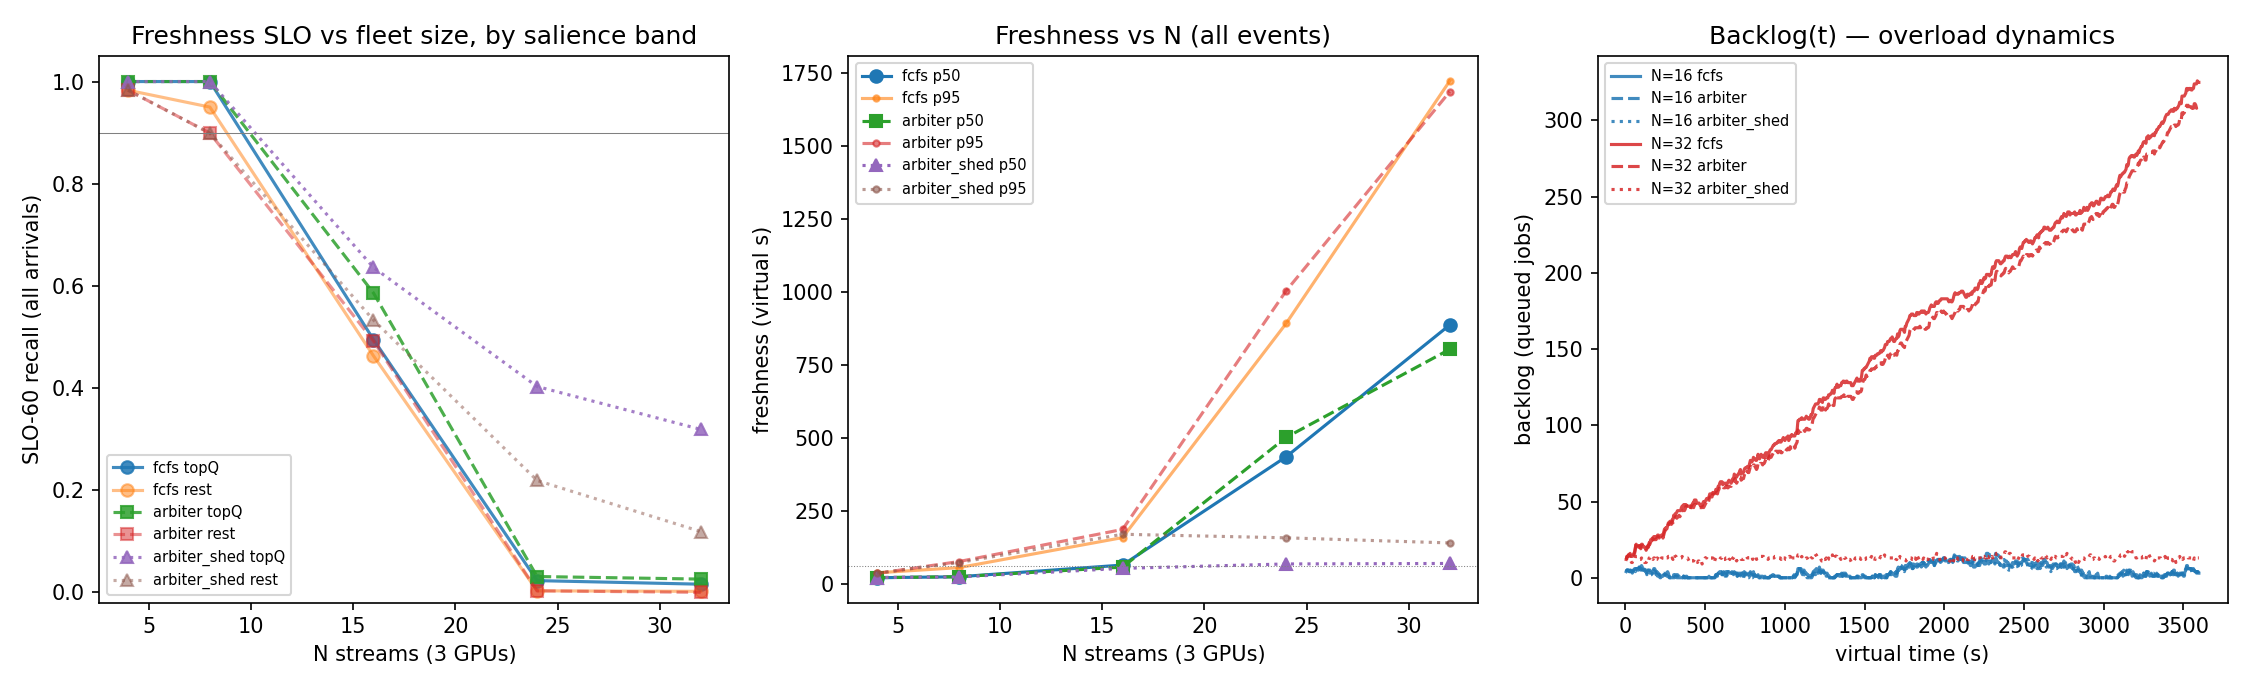
\includegraphics[width=\columnwidth]{figures/fleet_v1_curves.png}
\caption{Fleet v1: SLO-60 recall vs.\ fleet size per policy, split by salience band; backlog traces confirm the admission-control mechanism.}
\label{fig:fleet}
\end{figure}

\subsection{Eviction under a storage budget}
\label{sec:exp-eviction}

We sweep retention $\in \{50, 25, 10, 5, 2\}\%$ of the full-corpus memory (749 events) under five policies --- recency (FIFO), random, salience-only, coverage (ours), coverage+tombstones --- and re-run the 220 SMB queries per cell (36 cells; no new inference).

\begin{table}[t]
\centering
\caption{Eviction frontier, corrected reporting (61-cell matrix: policy $\times$ tombstones $\times$ budget; random = mean of 3 seeds). Existence accuracy is reported alone --- it collapses under eviction and balanced accuracy hides this (negation FAR mechanically falls as memory shrinks). Tombstones lift \emph{only} retrieval AP; with tombstones ON, all policies converge (AP 0.173--0.184 at 2\%), i.e., the stubs, not the selection, carry the aggregate signal.}
\label{tab:eviction}
\small
\begin{tabular}{@{}lcccc@{}}
\toprule
Policy & Existence @25\% & AP @25\% (OFF$\to$ON) & AP @10\% (OFF$\to$ON) & AP @2\% (OFF$\to$ON) \\
\midrule
None (100\%) & \textbf{0.950} & \multicolumn{3}{c}{AP 0.353 (no eviction)} \\
\midrule
Recency (FIFO) & 0.183 & .163 $\to$ .178 & .077 $\to$ .125 & .047 $\to$ \textbf{.184} \\
Salience & 0.283 & .177 $\to$ .200 & .074 $\to$ .118 & .052 $\to$ \textbf{.184} \\
Coverage (ours) & \textbf{0.333} & .091 $\to$ .162 & .053 $\to$ .122 & .027 $\to$ .173 \\
Random & 0.350 & .148 $\to$ .182 & .066 $\to$ .116 & .044 $\to$ .176 \\
\bottomrule
\end{tabular}
\end{table}

Findings (Figure~\ref{fig:eviction}): (i) \textbf{point queries collapse under eviction regardless of policy} --- existence accuracy falls from 0.950 to 0.18--0.35 at 25\% retention, a fact our earlier balanced-accuracy reporting had hidden (the negation-FAR confound); (ii) without tombstones, selection policy matters for breadth --- coverage retains the most rare events (GT coverage 0.352 vs.\ recency's 0.302 at 25\%) and the best balanced accuracy; (iii) \textbf{tombstones rescue aggregate answerability but equalize policies}: retrieval AP at 2\% retention rises 3.5$\times$ against the strongest selection policy (salience, 0.052$\to$0.184) and 6.4$\times$ against the weakest (coverage, 0.027$\to$0.173), with all policies converging to 0.173--0.184 --- eviction as compression works, but the compression, not the selection, does the work; (iv) the tombstone gain is budget-dependent: large at 2--10\%, negligible at 50\%.

\begin{figure}[t]
\centering
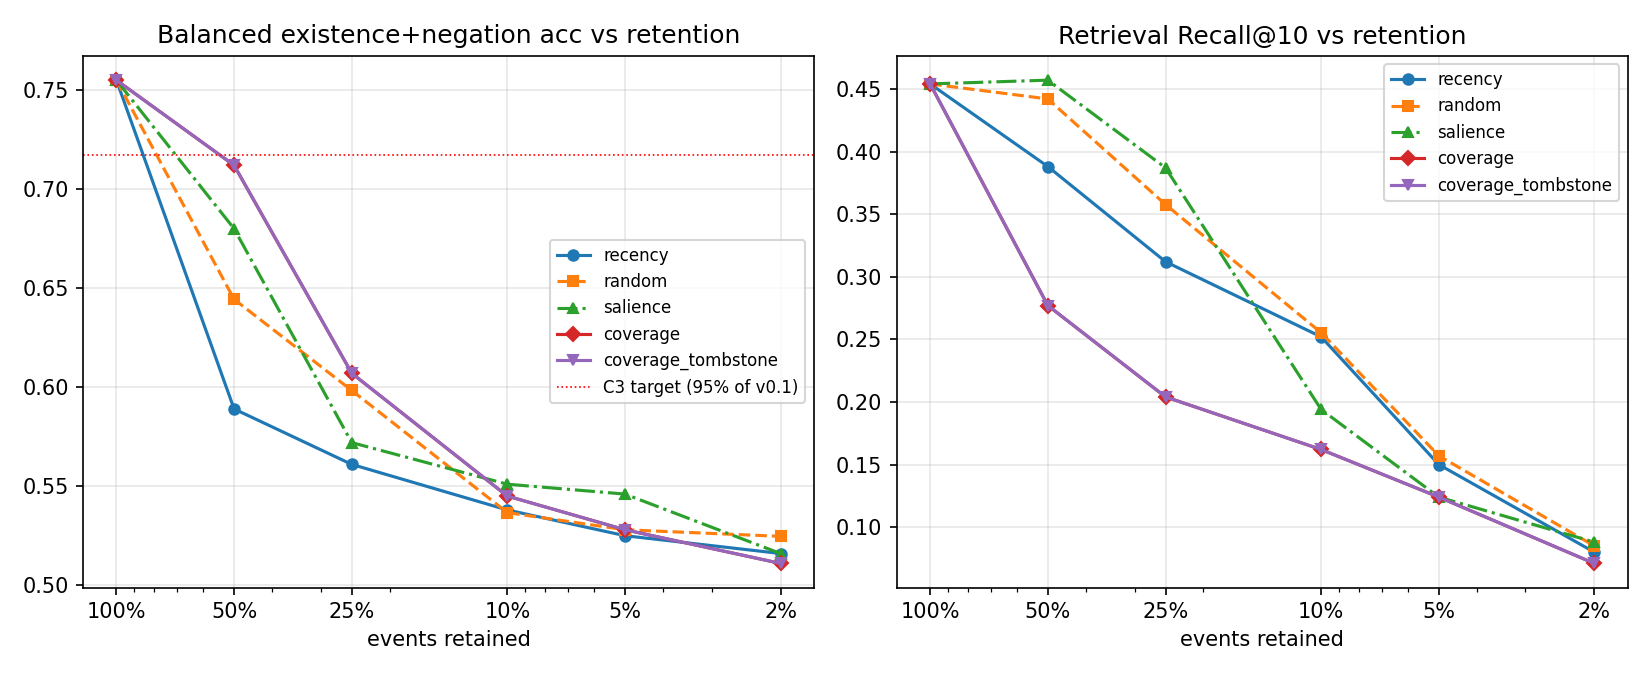
\includegraphics[width=\columnwidth]{figures/eviction_frontier.png}
\caption{Eviction frontier: query accuracy vs.\ retention budget per policy.}
\label{fig:eviction}
\end{figure}

\subsection{Appearance vs.\ event semantics: TASTI-lite}
\label{sec:exp-tasti}

TASTI-lite instantiates the classical semantic index in our setting: CLIP ViT-B/16 embeddings~\cite{clip} of 4{,}944 uniform 30-s chunks, text-encoder queries, threshold calibrated on the same frozen split, identical metrics code. It is deliberately given more raw coverage than \sys (every chunk embedded).

\begin{table}[h]
\centering
\caption{Appearance-only memory vs.\ text+tag memory (same 220 queries). The E0 appearance-signature finding holds in-system.}
\label{tab:tasti}
\small
\begin{tabular}{@{}lcc@{}}
\toprule
 & TASTI-lite & \sys v0.1 \\
\midrule
Existence acc & 0.583 & \textbf{0.950} \\
Negation FAR & \textbf{0.200} & 0.440 \\
Temporal tIoU & 0.167 & \textbf{0.286} \\
Retrieval R@10 / AP & 0.269 / 0.157 & \textbf{0.454 / 0.353} \\
\bottomrule
\end{tabular}
\end{table}

Appearance embeddings lack event semantics (Table~\ref{tab:tasti}) --- the same conclusion our cross-camera analysis reached offline (label agreement 0.55--0.59 vs.\ 0.501 chance; Appendix~\ref{app:e0}) --- now demonstrated in a running system. Its only win (negation FAR 0.20) is mechanical: an under-triggering index false-alarms less.

\subsection{Generality: beyond surveillance}
\label{sec:exp-generality}

To test whether the write-cost principle is surveillance-specific, we run RVS-Ego (ReKV's native benchmark) with three systems: ReKV-0.5B, uniform captioning, and \emph{novelty-gated writes} --- \sys's ladder with a domain-neutral CLIP-delta gate in place of the anomaly signal.

\begin{table}[h]
\centering
\caption{Generality arm (RVS-Ego, 120 questions, token-F1; GPT-judge unreachable offline --- relative comparison only). The gating principle generalizes; caption memory is lossy for fine-grained procedural QA (Section~\ref{sec:discussion}).}
\label{tab:generality}
\small
\begin{tabular}{@{}lccc@{}}
\toprule
System & token-F1 & Write GPU-s/stream-h & GPU-s/query \\
\midrule
ReKV-0.5B (native) & \textbf{0.212} & 341 & 0.88 \\
Uniform writes & 0.143 & 851 & 0.91 \\
Novelty-gated (ours) & 0.130 & \textbf{418} & 0.88 \\
\bottomrule
\end{tabular}
\end{table}

The event-driven write principle transfers (half the write cost of uniform at comparable accuracy, no domain model); the caption representation does not dominate on fine-grained procedural QA, where full-fidelity KV retrieval wins. Section~\ref{sec:discussion} draws the design conclusion (a hybrid memory with an optional KV tier).

\section{Discussion}
\label{sec:discussion}

\paragraph{What the negative results taught us.} This project's design emerged from killing naive mechanisms, and we consider the negative results as load-bearing as the positive ones. (i) \emph{Priority ordering without admission control is useless under saturation} (Section~\ref{sec:exp-fleet}) --- a work-conservation result that redirects scheduler design from ordering to shedding. (ii) \emph{Appearance embeddings fail as event memory}, offline (cross-camera label agreement 0.55--0.59 vs.\ 0.501 chance) and in-system (Table~\ref{tab:tasti}) --- memory records must carry event semantics. (iii) \emph{VLMs are near-useless as online anomaly scorers} ($\Delta$AUC $\le +0.0009$ over tier-1, alarmist with more context; Appendix~\ref{app:e0}) but \emph{effective as gated narrators} (95.5\% grounded; Table~\ref{tab:grounded}) --- the same model class, two roles, opposite verdicts; the role assignment is the design. (iv) \emph{Per-window causal adaptation captures 0\% of oracle headroom} (Appendix~\ref{app:e0}), which is why the fleet arbiter is a slow controller over write rates rather than a per-window predictor.

\paragraph{Threats to validity.} (i) VLM-direct matches \sys's balanced accuracy on video-scoped queries (Section~\ref{sec:exp-baselines}); our differentiation is economic (7.4 GPU-s/query forever vs.\ $\approx$0) and structural (no corpus queries, no memory) --- readers should weigh accuracy parity against operating cost. (ii) Tier-1 salience is replayed from causally-computed score files, not recomputed live; its measured cost is charged, but a fully live tier-1 integration remains engineering. (iii) The fleet study is a virtual-time simulator with real GPU work, not a deployment; absolute fleet numbers depend on the acceleration and event-rate assumptions we document. (iv) \smb v0's known limits: no SHT normal videos (negation there uses taxonomy mismatch), video-level XD category attribution, query-after-ingest only. (v) The generality arm uses token-F1 in place of RVS's GPT-judge (unreachable offline); absolute levels are low and only relative comparison is meaningful. (vi) Negation FAR improves mechanically as memory shrinks; tight-budget accuracy numbers carry this caveat.

\paragraph{Open problems the experiments exposed.} Two of our pre-registered targets were missed, and both are research problems, not engineering debt. (1) \emph{Sub-event temporal precision}: tier-1 score plateaus saturate, and refined spans remain $\sim$3.5$\times$ ground-truth length (tIoU 0.286 vs.\ target 0.40). Finer temporal grounding likely needs a different signal (motion boundaries, narrated sub-spans) than detector plateaus. (2) \emph{The confirmation/abstention frontier}: verification fixes hallucinated confirmations (FAR 0.44$\to$0.08) but destroys genuine confirmation (0.95$\to$0.50--0.60) because narrations are generic while queries use category vocabulary; closing this gap (better write-time specificity, calibrated verifier confidence) is a real direction.

\paragraph{Toward hybrid memory.} The generality arm shows caption memory is lossy for fine-grained procedural QA, where full-fidelity KV retrieval wins accuracy (0.212 vs.\ 0.130 token-F1) at 34$\times$ the storage. A principled architecture follows: text/tag records as the semantic tier (cheap, queryable, fleet-wide), with an optional per-stream KV tier~\cite{rekv,livevlm} for detail, both under one budget. The eviction and admission machinery this paper builds applies to both tiers unchanged.

\paragraph{Generalizability of the economics.} Our absolute numbers are V100-era; the \emph{ratios} (event-driven vs.\ time-driven write cost, MB vs.\ GB per stream-day, ordering vs.\ admission control) are architectural and should transfer to newer hardware, since all systems compared share the same hardware in our evaluation.

\section{Conclusion}
\label{sec:conclusion}

Always-on video fleets need memory that is persistent, queryable, and affordable. Existing systems leave this unsolved in a specific way: none of them treat memory as a budgeted resource. \sys does --- with event-driven writes (2.7$\times$ cheaper GPU at equal recall), tombstoned eviction (3.5$\times$ better aggregate answerability than the strongest delete-only policy at 2\% storage), admission control that holds freshness SLOs for important events where fair queueing collapses (10--20$\times$), and a query path that can abstain. Evaluated on \smb, our cost-instrumented surveillance memory benchmark, \sys leads every accuracy metric among memory systems at $\approx$0 GPU-s per query and $\sim$10$^4$--$10^5\times$ less storage than KV-state retention (depending on the competitor's compression setting). More broadly, we hope the cost-accounting discipline of this paper --- GPU-seconds per camera-hour, bytes per stream-day, accuracy-vs-cost frontiers --- becomes standard in a literature that currently reports none of them. Code, benchmark, and per-run reproducibility artifacts are released (Appendix~\ref{app:repro}).


\bibliographystyle{ACM-Reference-Format}
\bibliography{references}

\appendix
\section{Prior Measurement Study (E0) Informing the Design}
\label{app:e0}

\sys's design decisions are justified by a measurement study we conducted on the same hardware and datasets before building the system. We summarize the load-bearing numbers; each is replicated across two datasets (UCF-Crime, XD-Violence) and, where applicable, two VLM families (Holmes-VAU-2B~\cite{holmesvau}, VERA/InternVL2-8B~\cite{vera,internvl}).

\paragraph{Pipeline cost census (E0.8).} Per camera-hour: decode 0.6\% of GPU budget (25{,}482 frames/s on 16 CPU cores); tier-1 CLIP feature extraction 46.1\% (305 frames/s, 354 GPU-s); tier-1 head 0.1\%; VLM escalation at an 8.6\% rate 53.2\%. A server carries 19 cameras with the VLM stage vs.\ 40 without.

\paragraph{VLM as scorer: near-zero value.} Escalating uncertain clips to a VLM changes frame-level AUC by $+0.0009$ raw / $-0.0006$ calibrated against a $+0.0256$ oracle ceiling on 5{,}965 escalated clips (2--4\% of headroom). The VLM's ``93.4\% accuracy'' on the pool is a base-rate artifact (a constant ``No'' scores 93.58\%). More context makes the VLM \emph{more} alarmist (within-pool ranking AUC 0.669$\to$0.605 as context grows 0.5\,s$\to$34\,s); a second VLM family reproduces the failure (band capture $-10.8\%$, within-pool AUC 0.470, below random). \emph{Design consequence: the VLM narrates; it never scores.}

\paragraph{Tier-1 oversampling.} Zero-order-hold stride sweep: stride 1 = 0.8802 AUC / 359.3 GPU-s; stride 4 = 0.8788 / 89.8; stride 8 = 0.8763 / 44.9; stride 16 = 0.8704 / 22.5. Tier-1 is 4--8$\times$ oversampled for detection.

\paragraph{Workload burstiness.} Demand exceeds capacity at $N$=16 cameras (p95) / $N$=32 (mean) on 4$\times$V100, robust across a 4$\times$ clip-period swing and replicated on XD-Violence; burstiness p95/mean = 2.77. Fleets live near saturation --- hence the arbiter.

\paragraph{Semantic verdict cache: dead as designed.} Raw ``safe hit rate'' reaches 99.9\%, but under a base-rate-invariant criterion (suppressed anomalies $\le$1\%) the safe hit rate is 5.7\% at threshold 0.99; $\ge$96\% of hits are same-video temporal reuse, 94.4\% within one minute; the cache's marginal value over a gate is $\sim$14\% of escalated calls (capacity multiplier 1.16$\times$). \emph{Design consequence: no verdict cache; temporal redundancy is exploited by the write gate instead.}

\paragraph{Appearance signatures fail for events.} Cross-camera neighbors at similarity $\ge$0.80 agree on labels at 0.55--0.59 vs.\ 0.501 chance (ShanghaiTech); appearance encodes scene, not event content. \emph{Design consequence: memory records carry text + score trajectories; appearance embeddings are excluded from retrieval keys (confirmed in-system, Section~\ref{sec:exp-tasti}).}

\paragraph{Per-window adaptation fails.} A causal per-window sampling controller captures 0\% of measured oracle headroom on both datasets (predictor--outcome correlation $\approx$0 on UCF). \emph{Design consequence: adaptation lives at fleet granularity (the arbiter), not per window.}

\section{Per-System Profiles Behind Table~\ref{tab:gap}}
\label{app:profiles}

Each profile below was extracted from a full-text read of the cited paper in September 2026; ``not stated'' means the paper reports nothing on the axis.

\textbf{ReKV}~\cite{rekv}: stores full-fidelity per-frame KV offloaded to RAM/disk + per-frame retrieval keys; 18.8\,GB/h (7B) / 4.0\,GB/h (0.5B) at 0.5\,FPS; 11\,FPS encode on A100; fixed $r$=64 retrieved frames per query; single stream, $\le$1\,h horizons; its appendix calls surveillance-scale cache growth ``unsustainable.''

\textbf{LiveVLM}~\cite{livevlm}: compressed KV only (vision-sink bucketing, 12k-token cap); permanent discard, offload disabled by design; validated on one 24\,GB consumer GPU; retrieval over KV pages improves accuracy vs.\ full cache (68.1 vs.\ 66.2 MLVU) via redundancy filtering.

\textbf{StreamMem}~\cite{streammem}: saliency-pruned KV at 6K tokens/layer; query-agnostic; the only real eviction policy in the set, but GPU-resident and per-video.

\textbf{StreamingVLM}~\cite{streamingvlm}: 512 text tokens + 16\,s vision window is the entire long-term memory; recency-only eviction; 8\,FPS on one H100; no retrospective querying is possible by construction.

\textbf{Avas}~\cite{avas}: event knowledge graph (five tables) + per-frame embeddings + retained raw frames; a 7B VLM captions every 3-s chunk unconditionally; indexing throughput 2.5\,FPS on one RTX\,3090 vs.\ 2\,FPS input; query latency $\sim$3--4\,min; no bytes/hour anywhere.

\textbf{VideoRAG}~\cite{videoraghkuds}: knowledge graph + text-chunk embeddings + one visual embedding per 30-s clip; every clip captioned and transcribed; unbounded graph growth; accuracy-only evaluation (win-rates 52--58\% on subjective axes).

\textbf{WorldMM}~\cite{worldmm}: textual knowledge graphs at four temporal scales + semantic KG + retains every sampled frame; driven by paid API models; no cost numbers at all (not even token counts); week-long single-video horizon (44.3\,h).

\textbf{VideoDB}~\cite{videodb}: strict-JSON scene artifacts from a VLM call every 5-s scene per stream + derived text embeddings; ``append-mostly'' memory; cost measurement explicitly deferred to future work; retrieval-quality evaluation only.

\section{SMB Construction Details}
\label{app:smb}

Event inventories are rebuilt from official label files (UCF \texttt{Temporal\_Anomaly\_Annotation.txt}; XD \texttt{annotations.txt} + filename category codes; SHT \texttt{test\_frame\_mask/*.npy}), never from our own model outputs. Queries are template-instantiated from the inventories (category names, video ids, camera ids, time spans), then paraphrased (temperature 0.7) with the deterministic template preserved per query. Difficulty strata combine event duration (short/long) with peak tier-1 score (high/low). The QC script recomputes every ground-truth artifact from raw labels and checks each query against it. Counts: UCF 290 videos / 10.3\,h / 156 events (top categories: Shooting 25, Shoplifting 25, RoadAccidents 23); XD 800 / 27.0\,h / 1{,}238 (Car Accident 513, Fighting 275, Shooting 261); SHT 107 / 0.45\,h / 194 events across 12 cameras.

\section{Groundedness Methodology}
\label{app:grounded}

Judging is cross-family (each model's narrations judged against frames by the other model family) to avoid self-agreement bias; judges answer three binary questions (actions supported? hallucinated content? usable as memory entry?) with strict JSON at temperature 0.1. Label-anchored checks use a documented keyword map per category (e.g., Robbery$\to$\{steal, grab, snatch\}) for consistency on anomalous events, and a strict violence-keyword map for false-alarm detection on normal events (a loose vocabulary would inflate false alarms to 32--40\% via benign matches like parade ``rifles''; the strict map yields 0--7.5\%). Judge leniency asymmetry (InternVL2-as-judge approves 99.5\% of Qwen's narrations) is documented; we rely on orderings, not absolute rates.

\section{Volta Porting Notes}
\label{app:porting}

All systems ran on Tesla V100 (sm\_70, fp16, no FlashAttention-2). We found and fixed a genuine upstream bug: ReKV-lineage's torch fallback attention computes QK$^{\top}$ and softmax entirely in fp16, which saturates at head\_dim 128 (Qwen2-7B) and produces degenerate output; upstream never observed it because their H800s used the triton kernel, which upcasts. Our two-line fp32-upcast patch fixes 7B output; the same bug exists verbatim in MuKV. LiveVLM required routing its streaming attention (registered only under \texttt{flash\_attention\_2}) to SDPA with a bottom-right causal mask. Qwen2.5-VL's vision SDPA builds a dense $N^2$ mask; frames are pre-resized to multiples of 28. All patches are preserved (Appendix~\ref{app:repro}).

\section{Reproducibility}
\label{app:repro}

Every experiment is a run directory containing: \texttt{config.json} (written before the run, never edited), \texttt{env.json} (conda environment + full package list), \texttt{code\_state.json} (commit hashes + patch files for every external repository), \texttt{data\_manifest.json}, logs, \texttt{metrics.jsonl}, and \texttt{cost.json} (GPU-seconds per stage, wall time, peak VRAM). Failed runs are retained and marked. An append-only experiment log indexes all runs, including four pre-convention ones (baseline validation, narration spike, groundedness, benchmark construction). Baseline pins: ReKV commit \texttt{1fd9a3d}; LiveVLM commit \texttt{8b84be8}; Qwen2.5-VL via transformers 4.49.0. The calibration split (frozen 20\% of SMB queries) is shared by all systems that need a threshold.


\end{document}
